% !TeX program = xelatex
\documentclass[12pt,a4paper]{article}

\usepackage{fontspec}
\usepackage[turkish]{babel}
\AtBeginDocument{\shorthandoff{=}} % tikz key=value seçenekleri için
\usepackage{amsmath,amssymb}
\usepackage{geometry}
\usepackage{tikz}
\usepackage{xcolor}
\usepackage{enumitem}
\setmainfont{Latin Modern Roman}

\geometry{margin=2.5cm}

\definecolor{TitleColor}{HTML}{0B3C5D}
\definecolor{QuestionColor}{HTML}{0D3B66}
\definecolor{ChoiceColor}{HTML}{8A2D12}

\renewcommand{\labelenumi}{\textbf{\color{QuestionColor}\arabic{enumi}.}}
\renewcommand{\labelenumii}{\textbf{\color{ChoiceColor}(\alph{enumii})}}

\setlist[enumerate,1]{leftmargin=*,font=\bfseries\color{QuestionColor}}
\setlist[enumerate,2]{leftmargin=1.2cm,font=\bfseries\color{ChoiceColor}}
\setlist[itemize]{leftmargin=1.2cm,font=\bfseries\color{ChoiceColor},label=\textbf{\color{ChoiceColor}$\blacktriangleright$}}

\title{\textbf{\color{TitleColor}Olasılık -- Toplu Ödev Çözümleri}}
\author{}
\date{}

\newcommand{\C}[2]{\binom{#1}{#2}}

\begin{document}
\maketitle

\section*{\textbf{\color{TitleColor}Cevaplar}}

\begin{enumerate}
\item Seçimler iki bağımsız kombinasyon adımından oluşur:
\[
N=\binom{8}{4}\binom{6}{2}.
\]
\[
\binom{8}{4}=70,\qquad \binom{6}{2}=15
\quad \Rightarrow \quad
N=70\cdot 15=1050.
\]
\[
\boxed{N=1050}
\]

\item Koşul olayı
\[
E=\{2,4,6\}
\]
olduğundan örnek uzay $E$ ile sınırlandırılır.
\begin{center}
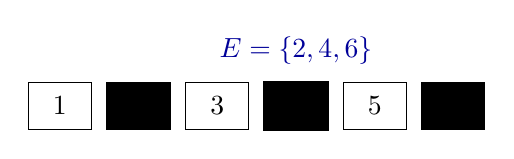
\begin{tikzpicture}
\draw (0,0) rectangle (0.8,0.6); \node at (0.4,0.3) {1};
\draw[fill=blue!10] (1.0,0) rectangle (1.8,0.6); \node at (1.4,0.3) {2};
\draw (2.0,0) rectangle (2.8,0.6); \node at (2.4,0.3) {3};
\draw[fill=orange!20,thick] (3.0,0) rectangle (3.8,0.6); \node at (3.4,0.3) {4};
\draw (4.0,0) rectangle (4.8,0.6); \node at (4.4,0.3) {5};
\draw[fill=blue!10] (5.0,0) rectangle (5.8,0.6); \node at (5.4,0.3) {6};
\node[blue!60!black] at (3.4,1.0) {$E=\{2,4,6\}$};
\end{tikzpicture}
\end{center}
\begin{enumerate}
\item
\[
P(X=4\mid E)=\frac{P(\{4\}\cap E)}{P(E)}=\frac{1/6}{3/6}=\frac{1}{3}.
\]
\[
\boxed{P(X=4\mid X\in\{2,4,6\})=\frac{1}{3}}
\]
\item Başlangıçta örneklem uzayı
\[
\Omega=\{1,2,3,4,5,6\}
\]
olup $|\Omega|=6$ idi ve her sonuç eş olasılıklıydı. ``Sonuç çifttir'' koşulu verildiğinde artık yalnızca bu koşulla uyumlu sonuçlar mümkün kabul edilir:
\[
E=\{2,4,6\},\qquad |E|=3.
\]
Dolayısıyla olasılık hesabı $\Omega$ üzerinde değil, daraltılmış uzay $E$ üzerinde yapılır. Bu nedenle payda $6$ yerine $3$ olur; yani koşullu olasılık, başlangıç uzayını bilgiye göre filtrelenmiş bir alt uzaya indirger.
\end{enumerate}

\item Verilenler:
\[
P(C)=0.30,\qquad P(R)=0.50,\qquad P(C\cap R)=0.18.
\]
Venn bölge olasılıkları:
\[
P(C\setminus R)=0.30-0.18=0.12,\qquad
P(R\setminus C)=0.50-0.18=0.32.
\]
\begin{center}
\begin{tikzpicture}[scale=0.95]
\draw[rounded corners=4pt] (-3.1,-2.2) rectangle (3.1,2.2);
\node at (-2.6,1.85) {$\Omega$};

\fill[blue!18] (-1.0,0) circle (1.35);
\fill[red!18] (1.0,0) circle (1.35);

\draw[thick,blue!60!black] (-1.0,0) circle (1.35);
\draw[thick,red!60!black] (1.0,0) circle (1.35);

\node at (-2.0,1.25) {$C$};
\node at (2.0,1.25) {$R$};

\node[fill=white,inner sep=1pt] at (-1.55,0) {$0.12$};
\node[fill=white,inner sep=1pt] at (0,0) {$0.18$};
\node[fill=white,inner sep=1pt] at (1.55,0) {$0.32$};
\end{tikzpicture}
\end{center}
\begin{enumerate}
\item
\[
P(R\mid C)=\frac{P(C\cap R)}{P(C)}=\frac{0.18}{0.30}=0.60.
\]
\[
\boxed{P(R\mid C)=0.60}
\]
\item
\[
P(C\mid R)=\frac{P(C\cap R)}{P(R)}=\frac{0.18}{0.50}=0.36.
\]
\[
\boxed{P(C\mid R)=0.36}
\]
\end{enumerate}

\item Verilenler:
\[
P(M)=0.50,\qquad P(O)=0.40,\qquad P(M\cap O)=0.20.
\]
Dahil etme-çıkarma kuralı:
\[
P(M\cup O)=P(M)+P(O)-P(M\cap O)=0.50+0.40-0.20=0.70.
\]
\begin{center}
\begin{tikzpicture}[scale=0.95]
\draw[rounded corners=4pt] (-3.1,-2.2) rectangle (3.1,2.2);
\node at (-2.6,1.85) {$\Omega$};

\fill[blue!18] (-1.0,0) circle (1.35);
\fill[red!18] (1.0,0) circle (1.35);

\draw[thick,blue!60!black] (-1.0,0) circle (1.35);
\draw[thick,red!60!black] (1.0,0) circle (1.35);

\node at (-2.0,1.25) {$M$};
\node at (2.0,1.25) {$O$};

\node[fill=white,inner sep=1pt] at (-1.55,0) {$0.30$};
\node[fill=white,inner sep=1pt] at (0,0) {$0.20$};
\node[fill=white,inner sep=1pt] at (1.55,0) {$0.20$};
\end{tikzpicture}
\end{center}
\[
\boxed{P(M\cup O)=0.70}
\]

\item Toplam parça sayısı $30$, kusurlu parça sayısı $3$.
\begin{center}
\begin{tikzpicture}[>=latex, line width=0.8pt]
\node (om) at (0,0) {$\Omega$};
\node (k1) at (3.0,1.3) {$K_1$};
\node (s1) at (3.0,-1.3) {$S_1$};
\node (k2) at (6.2,2.0) {$K_2$};
\node (s2) at (6.2,0.6) {$S_2$};

\draw[->,blue!70!black] (om) -- (k1) node[midway,above] {$\frac{3}{30}$};
\draw[->,gray!70] (om) -- (s1) node[midway,below] {$\frac{27}{30}$};
\draw[->,red!70!black] (k1) -- (k2) node[midway,above] {$\frac{2}{29}$};
\draw[->,blue!70!black] (k1) -- (s2) node[midway,below] {$\frac{27}{29}$};

\node[font=\small,align=left] at (6.6,-1.2) {$K$: kusurlu\\$S$: kusursuz};
\end{tikzpicture}
\end{center}
\begin{enumerate}
\item
\[
P(\text{1. parça kusurlu})=\frac{3}{30}=\frac{1}{10}.
\]
\item
Birinci parça kusurlu seçildiyse toplam parça sayısı $29$'a düşer ve kusurlu parça sayısı $2$ kalır (geri koyma yok).
Bu nedenle koşullu olasılık
\[
P(\text{2. parça kusurlu}\mid \text{1. parça kusurlu})=\frac{2}{29}.
\]
\item Çarpma kuralı:
``İki parça da kusurlu'' olayı, birinci parçanın kusurlu gelmesi ve bunun ardından ikinci parçanın (birinci kusurlu iken) kusurlu gelmesi olaylarının birlikte gerçekleşmesidir.
Bu yüzden
\[
P(K_1\cap K_2)=P(K_1)\,P(K_2\mid K_1)
\]
yazılır.
\[
P(\text{iki parça da kusurlu})
=\frac{3}{30}\cdot\frac{2}{29}
=\frac{1}{145}\approx 0.006897.
\]
\[
\boxed{P(\text{iki parça da kusurlu})=\frac{1}{145}\approx 0.006897}
\]
\end{enumerate}

\item Olaylar:
\[
T_1=\text{``1. transistör arızası''},\qquad T_2=\text{``2. transistör arızası''}.
\]
Seri devre, yalnızca iki transistör de sağlamsa çalışır:
\begin{center}
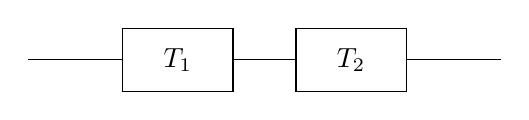
\begin{tikzpicture}
\draw (0,0) -- (1.2,0);
\draw (1.2,-0.4) rectangle (2.6,0.4);
\node at (1.9,0) {$T_1$};
\draw (2.6,0) -- (3.4,0);
\draw (3.4,-0.4) rectangle (4.8,0.4);
\node at (4.1,0) {$T_2$};
\draw (4.8,0) -- (6.0,0);
\end{tikzpicture}
\end{center}
\[
P(\text{çalışır})=P(T_1'\cap T_2')=(1-0.05)(1-0.08)=0.95\cdot 0.92=0.874.
\]
\[
P(T_1\cup T_2)=1-P(\text{çalışır})=1-0.874=0.126.
\]
\[
\boxed{P(\text{devre çalışmaz})=0.126}
\]

\item Olaylar:
\[
H_A=\text{A aşamasında hata},\quad
H_B=\text{B aşamasında hata},\quad
H_C=\text{C aşamasında hata}.
\]
Verilenler:
\[
P(H_A)=0.01,\qquad P(H_B)=0.02,\qquad P(H_C)=0.03.
\]
Parçanın tamamen hatasız olması için üç aşamada da hata olmamalıdır:
\[
H_A'\cap H_B'\cap H_C'.
\]
Aşamalar bağımsız olduğundan
\[
P(H_A'\cap H_B'\cap H_C')
=P(H_A')P(H_B')P(H_C')
=(1-0.01)(1-0.02)(1-0.03).
\]
\[
=0.99\cdot 0.98\cdot 0.97
=0.941094.
\]
\[
\boxed{P(\text{tamamen hatasız})=0.941094\approx 0.9411\ (\%94.11)}
\]

\item Olaylar:
\[
U=\text{istenen uzunluk},\quad X=\text{Metot X},\quad Y=\text{Metot Y}.
\]
\[
P(U\mid X)=0.80,\quad P(U\mid Y)=0.60,\quad P(X)=0.40,\quad P(Y)=0.60.
\]
\begin{center}
\begin{tikzpicture}[>=latex, line width=0.8pt]
\node (om) at (0,0) {$\Omega$};
\node (x) at (2.9,1.6) {$X$};
\node (y) at (2.9,-1.6) {$Y$};
\node (xu) at (5.9,2.35) {$U$};
\node (xuc) at (5.9,0.85) {$U'$};
\node (yu) at (5.9,-0.85) {$U$};
\node (yuc) at (5.9,-2.35) {$U'$};

\draw[->,blue!70!black] (om) -- (x) node[midway,above] {$0.40$};
\draw[->,gray!70] (om) -- (y) node[midway,below] {$0.60$};
\draw[->,blue!70!black] (x) -- (xu) node[midway,above] {$0.80$};
\draw[->,gray!70] (x) -- (xuc) node[midway,below] {$0.20$};
\draw[->,blue!70!black] (y) -- (yu) node[midway,above] {$0.60$};
\draw[->,gray!70] (y) -- (yuc) node[midway,below] {$0.40$};
\end{tikzpicture}
\end{center}
Toplam olasılık kuralı:
\[
P(U)=P(U\mid X)P(X)+P(U\mid Y)P(Y)
=0.80\cdot0.40+0.60\cdot0.60
=0.68.
\]
\[
\boxed{P(U)=0.68}
\]

\item Olaylar:
\[
D=\text{hasta},\qquad D'=\text{sağlıklı},\qquad +=\text{test pozitif}.
\]
\[
P(D)=0.02,\quad P(+\mid D)=0.95,\quad P(-\mid D')=0.90
\Rightarrow P(+\mid D')=0.10.
\]
\begin{center}
\begin{tikzpicture}[>=latex, line width=0.8pt]
\node (om) at (0,0) {$\Omega$};
\node (d) at (2.9,1.6) {$D$};
\node (dc) at (2.9,-1.6) {$D'$};
\node (dp) at (5.9,2.35) {$+$};
\node (dn) at (5.9,0.85) {$-$};
\node (dcp) at (5.9,-0.85) {$+$};
\node (dcn) at (5.9,-2.35) {$-$};

\draw[->,blue!70!black] (om) -- (d) node[midway,above] {$0.02$};
\draw[->,gray!70] (om) -- (dc) node[midway,below] {$0.98$};
\draw[->,blue!70!black] (d) -- (dp) node[midway,above] {$0.95$};
\draw[->,gray!70] (d) -- (dn) node[midway,below] {$0.05$};
\draw[->,blue!70!black] (dc) -- (dcp) node[midway,above] {$0.10$};
\draw[->,gray!70] (dc) -- (dcn) node[midway,below] {$0.90$};
\end{tikzpicture}
\end{center}
\[
P(+)=P(+\mid D)P(D)+P(+\mid D')P(D')
=0.95\cdot0.02+0.10\cdot0.98
=0.117.
\]
\[
P(D\mid +)=\frac{P(+\mid D)P(D)}{P(+)}
=\frac{0.95\cdot0.02}{0.117}
\approx 0.162.
\]
\[
\boxed{P(D\mid +)\approx 0.162}
\]

\item Verilenler:
\[
P(Y)=0.40,\qquad P(O)=0.35,\qquad P(Y\cap O)=0.25.
\]
Ayrık alt gruplar:
\[
P(\text{sadece }Y)=0.40-0.25=0.15,\quad
P(\text{sadece }O)=0.35-0.25=0.10,
\]
\[
P(Y\cap O)=0.25,\qquad
P(Y'\cap O')=1-\bigl(0.40+0.35-0.25\bigr)=0.50.
\]
\begin{center}
\begin{tikzpicture}[scale=0.95]
\draw[rounded corners=4pt] (-3.1,-2.2) rectangle (3.1,2.2);
\node at (-2.6,1.85) {$\Omega$};

\fill[blue!18] (-1.0,0) circle (1.35);
\fill[red!18] (1.0,0) circle (1.35);

\draw[thick,blue!60!black] (-1.0,0) circle (1.35);
\draw[thick,red!60!black] (1.0,0) circle (1.35);

\node at (-2.0,1.25) {$Y$};
\node at (2.0,1.25) {$O$};

\node[fill=white,inner sep=1pt] at (-1.55,0) {$0.15$};
\node[fill=white,inner sep=1pt] at (0,0) {$0.25$};
\node[fill=white,inner sep=1pt] at (1.55,0) {$0.10$};
\node[fill=white,inner sep=1pt] at (0,-1.55) {$Y'\cap O'=0.50$};
\end{tikzpicture}
\end{center}
Koşullu olasılıklar:
\begin{align*}
P(T\mid \text{sadece }Y)&=0.90,\qquad &P(T\mid \text{sadece }O)&=0.70,\\
P(T\mid Y\cap O)&=0.95,\qquad &P(T\mid Y'\cap O')&=0.10.
\end{align*}
\begin{enumerate}
\item Toplam olasılık:
\begin{align*}
P(T)&=0.90(0.15)+0.70(0.10)+0.95(0.25)+0.10(0.50)\\
&=0.135+0.070+0.2375+0.050\\
&=0.4925.
\end{align*}
\[
\boxed{P(T)=0.4925}
\]
\item Bayes:
\[
P(Y\cap O\mid T)=\frac{P(T\mid Y\cap O)P(Y\cap O)}{P(T)}
=\frac{0.95\cdot0.25}{0.4925}
\approx 0.4822.
\]
\[
\boxed{P(Y\cap O\mid T)\approx 0.4822}
\]
\item Bayes:
\[
P(Y'\cap O'\mid T)=\frac{P(T\mid Y'\cap O')P(Y'\cap O')}{P(T)}
=\frac{0.10\cdot0.50}{0.4925}
\approx 0.1015.
\]
\[
\boxed{P(Y'\cap O'\mid T)\approx 0.1015}
\]
\end{enumerate}
\end{enumerate}

\end{document}
